\documentclass[11pt]{article}            % Report class in 11 points
\parindent0pt  \parskip10pt             % make block paragraphs
\usepackage{graphicx}
\usepackage{listings}
\graphicspath{ {images/} }
\usepackage{graphicx} %  graphics header file
\begin{document}
\begin{titlepage}
    \centering
  \vfill
    
\includegraphics[width=8cm]{uni_logo.png} \\ 
	\vskip2cm
    {\bfseries\Large
	Data Structures and algorythm  \\ (CS09203)\\
	
	\vskip2cm
	Lab Report 
	 
	\vskip2cm
	}    

\begin{center}
\begin{tabular}{ l l  } 

Name: & MuhammadTalhaKhalid \\ 
Registration \#: &CSU-S16-135\\ 
Lab Report \#: & 3 \\ 
 Dated:& 13-04-2018\\ 
Submitted To:& Mr. Usman Ahmed\\ 

 %\hline
\end{tabular}
\end{center}
    \vfill
    The University of Lahore, Islamabad Campus\\
Department of Computer Science \& Information Technology
\end{titlepage}


    
    {\bfseries\Large
\centering
	Experiment \# 3 \\

Storing Data into stacks using Arrays using Stacks\\
	
	}    
 \vskip1cm
 \textbf {Objective}\\  To understand How to store Data using Stacks.
 
 \textbf {Software Tool} \\
1. Ubuntu Linux \\
2. Sublime text\\
3. g++\\

\section{Theory }              
In this experiment we store data into Array using the concept of stacks. First of all we push  44,55 and 77 into array then we display it after thet we pop the data from it and it remove 77 from array \\
Stacks has 2 rules:\\
1.	Only Enter single data at a time.\\
2.	Remove the last data which is your top .\\ \\


\section{Task}  
\subsection{Procedure: Task 1 }     

\begin{figure*}
\centering
  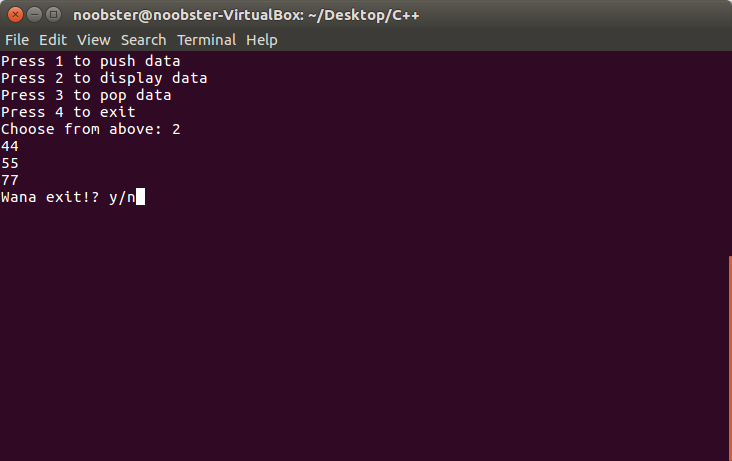
\includegraphics[width=12cm,height=6cm,keepaspectratio]{3.png}
\caption{4 numbers pushed into stacks}
\label{Figure:1}    
  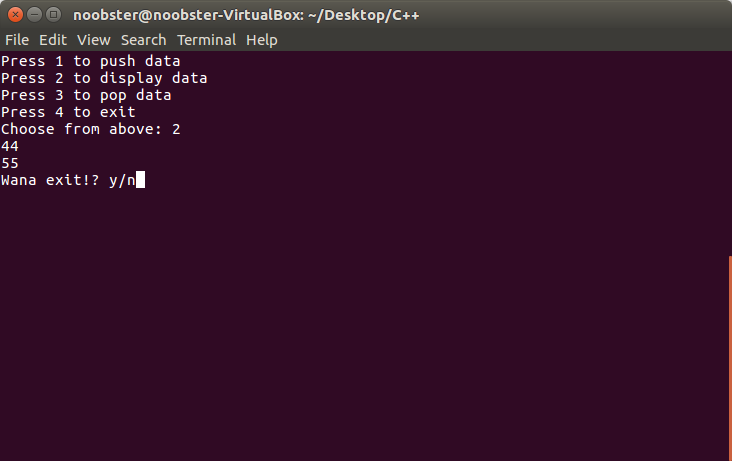
\includegraphics[width=12cm,height=6cm,keepaspectratio]{5.png}
\caption{1 number poped}
\label{Figure:2}   
\end{figure*}
We can pop  5 numbers into stacks the calling the function pop(); if numbers exceed the it will give error stacks overflow else it will ener data into it
If stack is empty then it will give error stack is empty else it wil wipe out all data from stacks

\subsection{Procedure: Task 2 }     

\begin{lstlisting}[language=C++]
#include<iostream>
#include<stdio.h>
#include <unistd.h>
#include<cstdlib>
using namespace std;
int top=-1;
int data[5];
int push(int inp) {
if(top==4) {
	cerr<<"Stack overflow!!\n";
	}else {
	data[++top]=inp;
	}
}
int  pop() {


if(top==-1) {
cerr<<"Stcack is empty!!\n";
	}else {
		cout<<data[top];
	top--;
}
}
void display() {
	for(int i=0;i<=top;i++) {
		cout<<data[i]<<endl;
	}
}
void list() {
	system("clear");
	cout<<"Press 1 to push data\n";
	cout<<"Press 2 to display data\n";
	cout<<"Press 3 to pop data\n";
	cout<<"Press 4 to exit\n";
}
int main() 
{
	int c1;
	int dtae;
	string choice="n";
	do {
	list();
	cout<<"Choose from above: ";
	cin>>c1;
	switch (c1) {
		case 1:
		do {
		cout<<"Enter data in numbers: ";
		cin>>dtae;
		push(dtae);
		cout<<"Wana continue?? y/n";
		cin>>choice;
	}while(choice!="y");
		break;

		case 2:
		do {
		display();

		cout<<"Wana exit!? y/n";
		cin>>choice;
	}while(choice!="y");
		break;
		case 3:
		do {
		pop();
		cout<<"Wana exit y/n";
		cin>>choice;
	}while(choice!="y");
		break;
	}
}while(c1!=4);
	

return 0;
}
\end{lstlisting}

\section{Conclusion}  
In this experiment we Push  data into stacks display it and then pop it  and we learn how to use stacks.
it is very usefull in many projects i have used stacks int  a small video game map designing proect of myne in which i store password of the door using stacks.
\end{document}                          % The required last line
